
\subsubsection{Gerade durch zwei gegebene Punkte}\index{Punkt auf Geraden}\index{Gerade!Punkt auf}
\TALS{Einstiegsaufgaben Frommenwiler: 606. a) c)}

Seien die Punkte $P=(10|6)$ und $Q=(-5|3)$ gegeben.
Gesucht ist die Funktionsgleichung $f: y=ax+b$ (namentlich $a$ und $b$), sodass
der Graph der Funktion $f$ durch beide Punkte führt.


\textbf{Rezept I: Graphisch}\\

\vspace{1mm}

\TNTeop{%%
\raisebox{2cm}{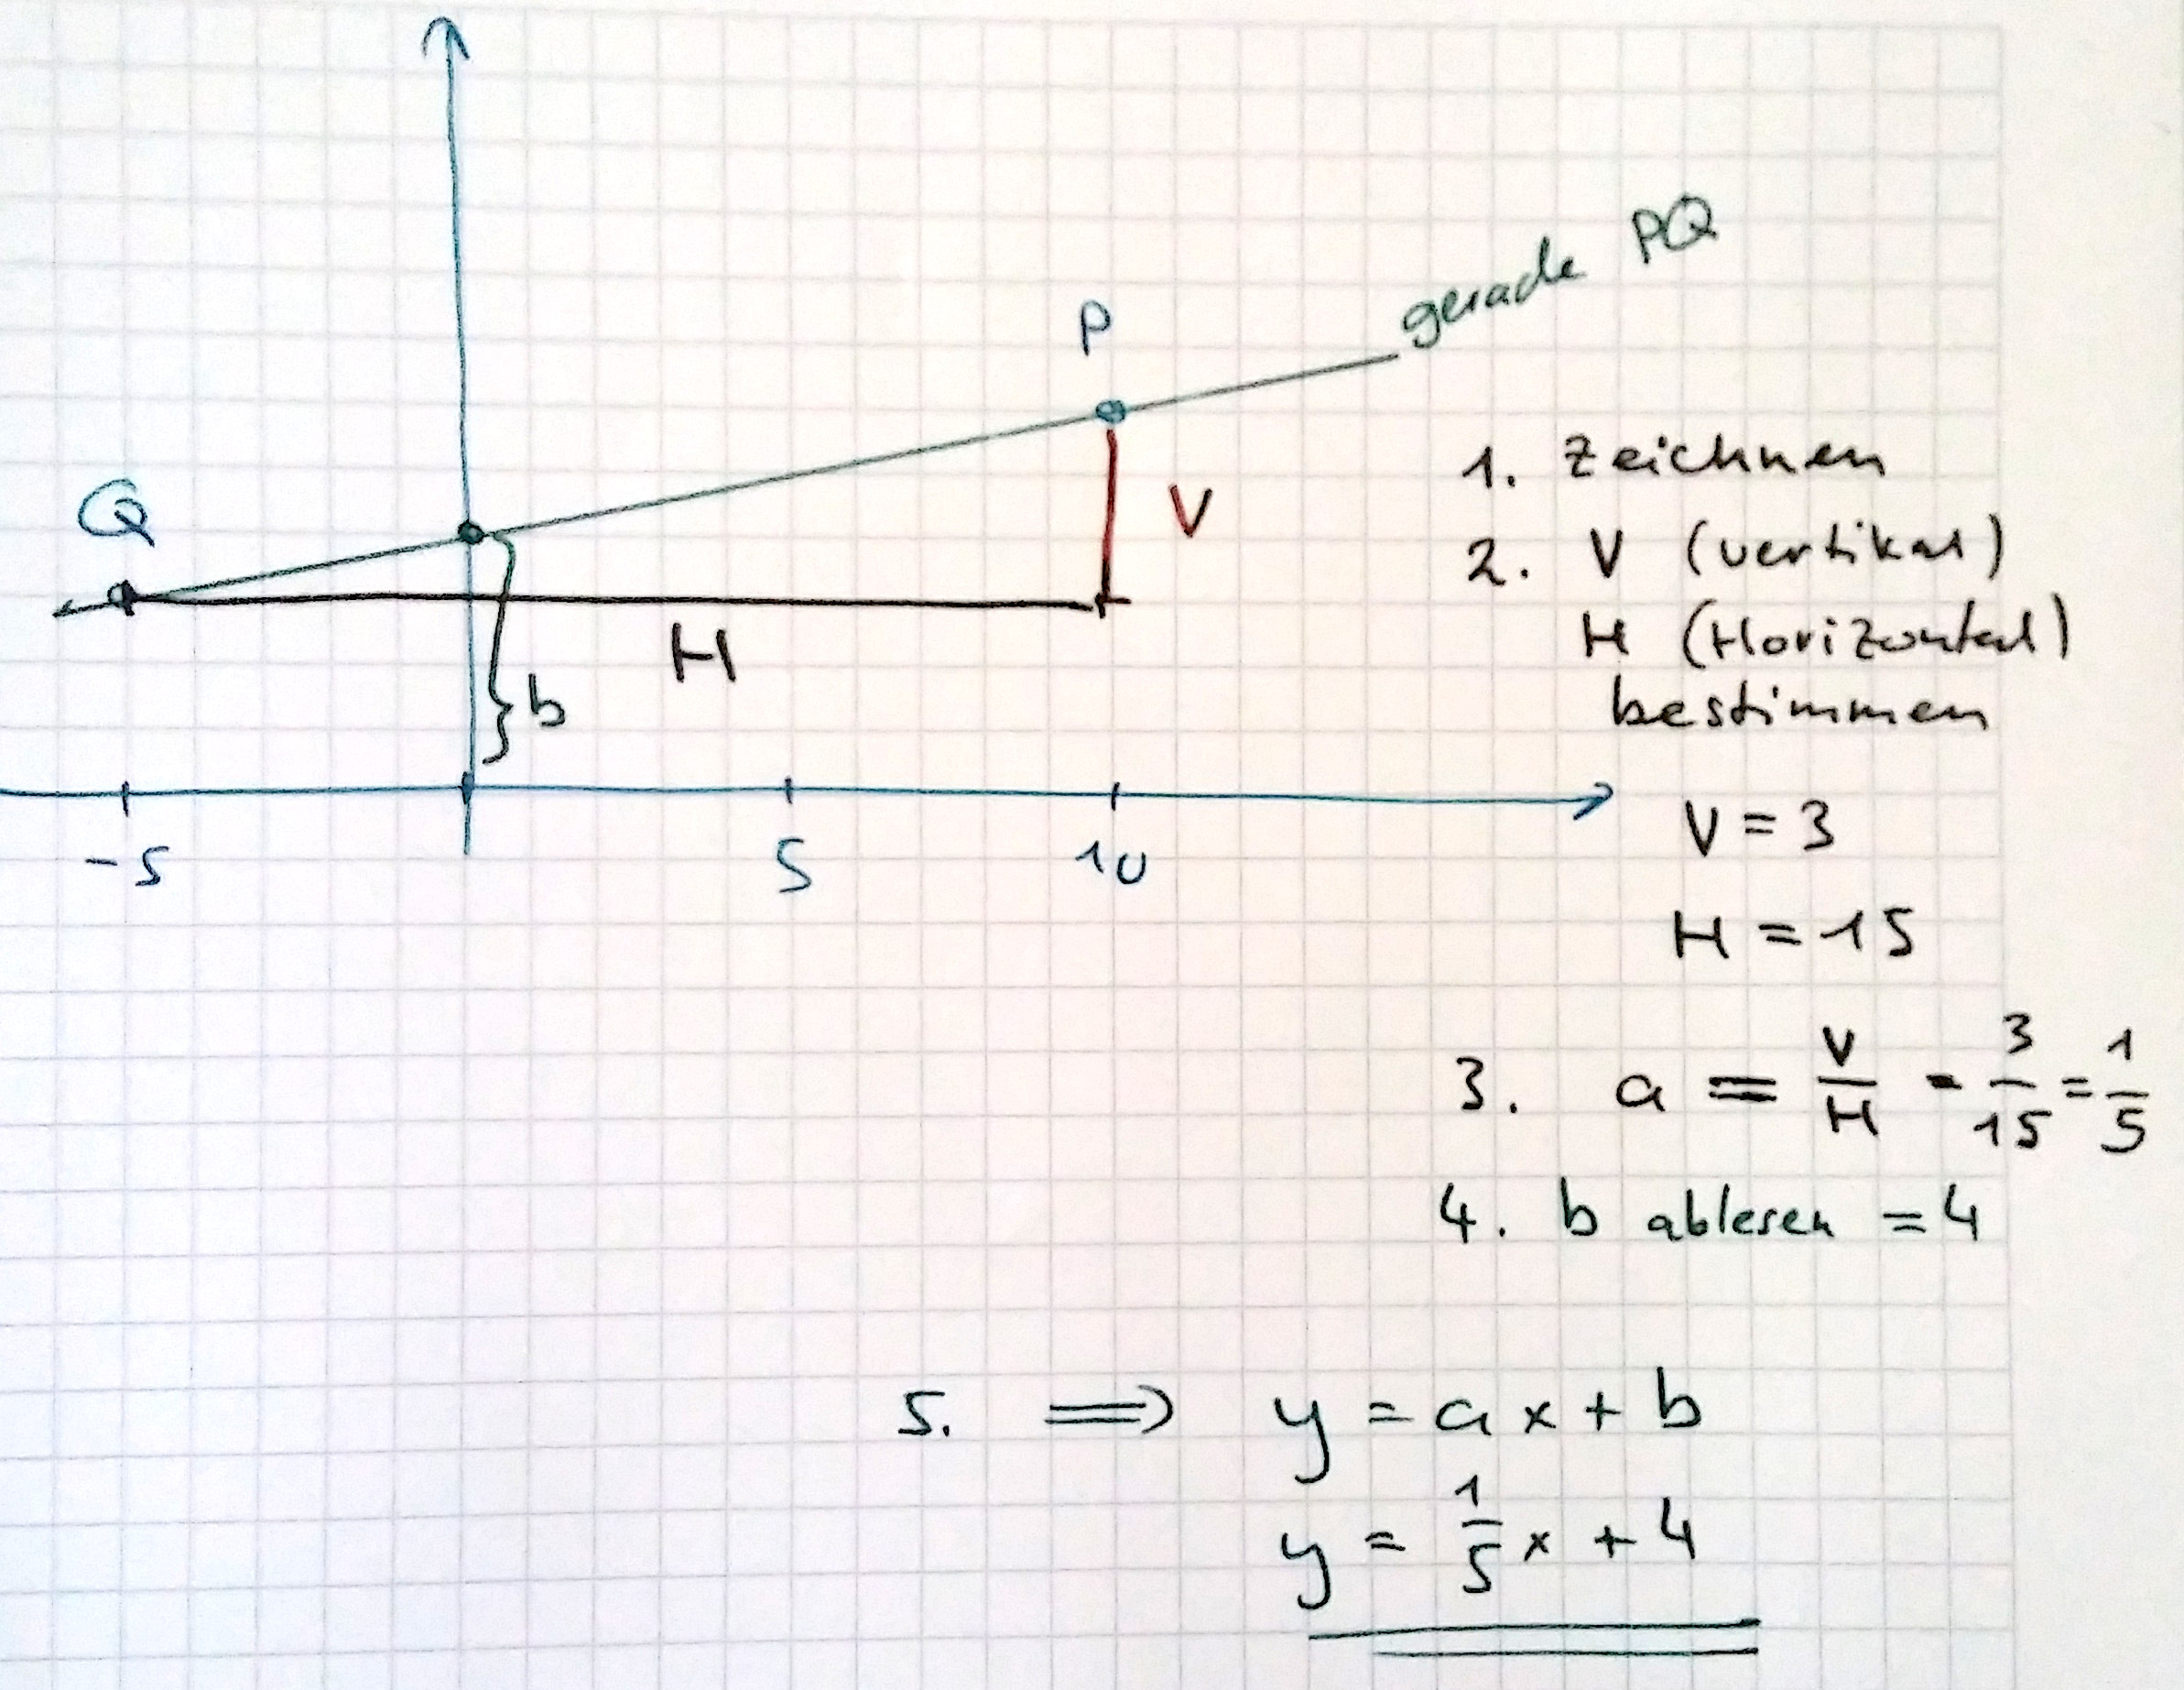
\includegraphics[width=16cm]{allg/funktionen/img/GeradeDurchZweiPunkte.jpg}}}%% END TNT EOP 


\textbf{Rezept II: Rechnerisch (algbraisch)}\\

\vspace{1mm}

\begin{rezept}{}{}
Um die Funktionsgleichung $$y=ax+b$$ zu finden,
  werden die $x$- und $y$-Koordinaten der beiden Punkte in die Gleichung eingesetzt und die beiden Gleichungen werden nach $a$ und $b$ aufgelöst. 
\end{rezept}

\TRAINER{
  TAFELText: Um $a$ und $b$ zu finden, setzen wir die $x$- und
  $y$-Koordinaten der beiden Punkte in die Funktionsgleichung ein.}
\noTRAINER{\vspace{12mm}}

Dies ergibt das folgende Gleichungssystem\footnote{Für $P$ gilt: $(x_P|y_P)=(x_P|f(x_P))=(x_P|ax_P+b)$ und somit $y_p =ax_P + b$.}:

\TNT{3.2}{\gleichungZZ%
{6}{a\cdot{}10 + b}%
{3}{a\cdot{}(-5) + b}
\vspace{1cm}
}%% END TNT

Die Subtraktion der beiden Gleichungen ergibt $3 = 15a$, was uns zu $a=\frac{1}{5}$ bringt.

Das $a$ kann auch durch das «Steigungsdreieck» berechnet werden:

$$a = \frac{y_Q-y_P}{x_Q-x_p} = \LoesungsRaumLang{\frac{3 - 6}{-5 - (-10)} = \frac{-3}{-15} = \frac{1}{5}}$$

Setzen wir $a=\frac{1}{5}$ in eine der beiden Gleichungen ein, so erhalten wir $b=4$. Die gesuchte Geradengleichung lautet also:

$$f: y=\LoesungsRaumLang{\frac{1}{5}\cdot{}x + 4}$$



\TALS{%%
Dies kann auch mit dem Taschenrechner gelöst werden; denn für alle Punkte $P$ auf $f$ gilt ja $P(x|y) = P(x|f(x))$:

$$f(x):=a\cdot{}x + b$$
\[
%%\begin{equation}%% but equation makes a number (1)
    gls:= \left\{\begin{array}{@{}lr@{}}
        f(10) = 6\\
        f(-5) = 3
        \end{array}\right.
\]
%%\end{equation}

  $$solve(gls,\{a, b\})$$
}%%

\GESOAadB{252ff}{15. a) c), 16. a), 18. a), 19., 25. a)}

\newpage

